\documentclass[12pt,fleqn]{article}\usepackage{../../common}
\begin{document}
Temel Fizik 2, Dönüşsel Kuvvet

İzafi Enerji Formülü

İzafi mekanikte kuvvet ve momentumdan başlayan formül biraz daha değişiyor [4].

$$
F = \frac{\ud (mv)}{\ud t}
$$

tanımında $m$'in değişmediğini farz etmiştik. Fakat izafi mekanikte enerji
uygulandıkça kütlenin büyüdüğünü göz önüne almak lazım. Bu büyüme faktörü
$\gamma = \left(1 - \frac{v^2}{c^2} \right)^{-1/2}$, yani bu faktöre oranla
kütle büyüyecek. Entegral şu hale geliyor,

$$
E_k = \int _{0}^{t} \frac{\ud (\gamma mv)}{\ud t} \ud x
$$

Bu entegral biraz daha karmaşık ama sonunda

$$
E_k = (\gamma - 1)mc^2
$$

elde ederiz. Yani kütleyi daha fazla hızlandırmak için gittikçe daha fazla iş
yapmak gerekir çünkü enerji eklendikçe kütle daha ağırlaşır. 

Dönüşler, Dönme Direnci (Moment of Inertia)

Saat yönü tersi yönde bir dönüş düşünelim, $s$ kadar dönüş olduysa, orijine
uzaklık $r$ ise, açısal mesafe [1, sf. 297]

$$
\theta = \frac{s}{r}
$$

ki $\theta$ radyan. Ya da

$$
s = r \theta
$$

Çemberin tamamı $2\pi$ rad (tam bir dönüş), meselâ 60 derece $\pi / 3$
rad. Çemberin çevresinin formülü $2\pi r$, eğer $\theta = \pi / 3$ rad ise,
$s = \pi / 3 \cdot r $.

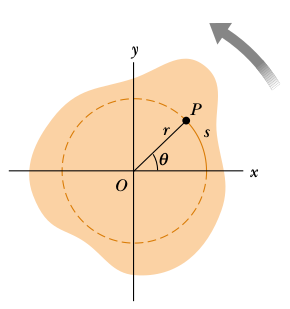
\includegraphics[width=15em]{phy_005_basics_08.png}

Açısal hızı bir $P$ noktasının teğetsel hızından yola çıkarak
hesaplayabiliriz, bu noktanın teğetsel hızı sonsuz ufak $s$'nin zamana göre
değişimi olacaktır, yani $v = ds / dt$, 

$$
v = \frac{ds}{dt} = r \frac{d\theta}{dt}
$$

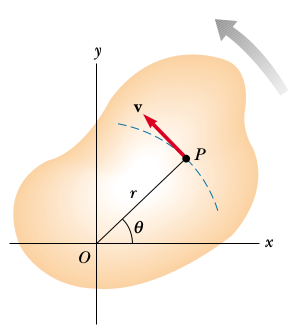
\includegraphics[width=15em]{phy_005_basics_09.png}

Elde edilen $d\theta / dt$ açısal değişimi gösteriyor, bu işte açısal
hızdır, ona $\omega$ diyelim, o zaman teğetsel hızı açısal hız ile şöyle
gösterebiliriz,

$$
v = r\omega
$$

Formül diyor ki dönen bir katı objenin herhangi bir noktasının teğetsel
hızı, o noktanın dönüş eksenine olan uzaklığı çarpı açısal hızına
eşittir. O zaman, her ne kadar katı objenin her noktası aynı açısal hızla
dönüyor olmasına rağmen her noktanın lineer hızı aynı değildir, çünkü $r$
her nokta için aynı değil. Üstteki formül dönüş merkezinden uzaklaştıkça
hızın artacağını söylüyor. Teğetsel hızı hayal etmek için o noktada ayakta
durabiliyor olsak yüzümüze çarpacak rüzgar hızını hayal edebiliriz. 

İvmeyi de dahil edelim, açısal ivme ile teğetsel ivmenin bağlantısına
bakalım, $v$'nin zamana göre türevini alırsak,

$$
a_t = \frac{dv}{dt} = r \frac{d\omega}{dt}
$$

$$
a_t = r \alpha
$$

Dönüşsel Kinetik Enerji

Dönmekte olan katı bir objenin kinetik enerjisini nasıl hesaplarız? 

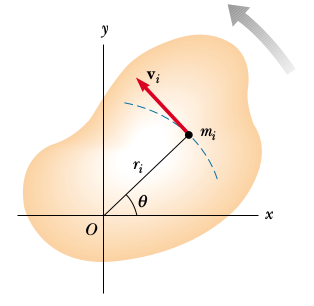
\includegraphics[width=15em]{phy_005_basics_10.png}

Objenin en ufak parçalarından başlayarak bunu yapmaya uğraşalım. Obje
$z$ ekseni etrafında dönüyor olsun, ve açısal hızı $\omega$
diyelim. Obje içindeki her parçacık $i$'nin kütlesi $m_i$ diyelim,
kinetik enerji bu parçacığın lineer hızına bağlıdır (objenin her
parçacığı aynı açısal hızda döner ama farklı noktalarda lineer hız
$v_i$ farklı olabilir, $v_i = r_i \omega$ üzerinden), o zaman her
parçacık için kinetik enerji [1, sf. 299]

$$
K_i = \frac{1}{2} m_i v_i^2
$$

ile gösterilebilir. Tüm obje için, 

$$
K_R = \sum_i K_i =
\sum_i \frac{1}{2} m_i v_i^2 =
\frac{1}{2} \sum_i m_i r_i^2 \omega^2
$$

Bu ifadede $\omega^2$'yi dışarı çekebiliriz, çünkü her parçacık için aynı,

$$
K_R = \frac{1}{2} \left( \sum_i m_i r_i^2 \right) \omega^2
$$

Parantez içindeki ifadeye bir isim verip değişken atayarak daha da işi
basitleştirebiliriz, bu ifadeye dönme direnci (moment of inertia) ismi
verilir,

$$
I \equiv  \sum_i m_i r_i^2
$$

$I$'nin birimi $kg \cdot m^2$'dir, bu notasyonla nihai denklem

$$
K_R = \frac{1}{2} I \omega^2
$$

haline gelir. 

Umarım lineer hareketin kinetik enerjisi $\frac{1}{2} m v^2$ ile dönüşsel
hareketteki kinetik enerji $\frac{1}{2} I \omega^2$ arasındaki benzerlik
dikkati çekmiştir. Lineerden dönüşsele geçerken / karşılaştırmalı
düşünürken $I$ hep $m$ yerine geçer, böyle görülür. Dönme direnci $I$ aynen
isminin çağrıştırdığı gibi bir kütlenin dönmeye olan gösterdiği dirençtir,
aynen bir objenin kütlesinin lineer harekete olan gösterdiği direnç olması
gibi. 

Önemli bir nokta daha, $I$ formülündeki $r_i$ dikkati çekmiştir, her $m_i$
parçacığının aynı birim ağırlıkta olduğunu farzetsek bile objenin farklı
noktalarında dönüş eksenine farklı uzaklıklar olabilir, yani bu uzaklıklar
objenin şekline göre değişik olacaktır. Mesela bir dikdörtgensel plakayı
orta noktasından döndürüyorsak ene ve boya olan uzaklıklar farklı
olacaktır. Bu sebeple tahmin edebileceğimiz üzere her obje için farklı $I$
hesabı olmalıdır. Bu hesabın detayları için [1, sf. 301]'e bakılabilir. İki
örnek obje için $I$ altta görülüyor.

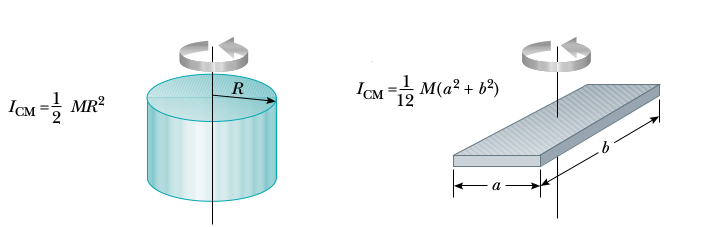
\includegraphics[width=25em]{phy_005_basics_11.png}

Tork (Torque)

Bir kuvvetin bir objeyi bir eksen etrafında döndürme kabiliyeti bir vektör
büyüklüğü olan tork ile ölçülür. Dönme eksenine olan uzaklık burada önemli
rol oynar, bir kapının kolu menteşeye olabildiği kadar uzaktır, çünkü
mesafe arttıkça aynı kuvvet ile daha fazla dönme, daha çok tork elde
edilir.

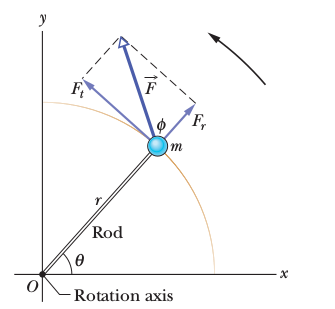
\includegraphics[width=15em]{phy_005_basics_12.png}

Tork her zaman dönme eksenine teğet olan kuvvet için hesaplanır, ve
uzaklık, kol uzaklığı, kuvvetin uygulandığı noktada eksene olan
uzaklıktır. Üstteki resimdeki tork $\tau$

$$
\tau = F \sin \phi = F d
$$

ile hesaplanır, ki $d = r \sin\phi$ olarak tanımladık.

Dikkat, tork türetilebilecek bir kavram değildir, bir tanımdır. Dönme
merkezine uzaklık çarpı kuvvet bazı kavramları biraraya getirmesi açısından
faydalı, bu sebeple kullanılıyor. 

Tork kuvvet ile karıştırılmamalı. Kuvvet lineer harekette değişiklik
yaratır, kuvvet dönüşsel harekette de değişiklik yaratır, ama bu tür
değişimde hem kuvvet hem de dönüş merkezine olan kol uzaklığı aynı oranda
rol oynar. 

Torkun birimi kuvvet çarpı uzunluk, yani Newton metredir. Diğer yandan
yapılan iş (work) ve torkun birimleri aynıdır, ama bu iki kavram da
birbirinden farklı.

Örnek

Çocuk parklarında tahtıravallı vardır, diyelim bir uçta şişman bir çocuk
biniyor, 10 Newton güç uyguluyor. Diğer yanda daha zayıf çocuk, o 5 Newton
güç uyguluyor. Bu tahtıravallı hala dengede durabilir, eğer dönme noktasına
şişman çocuk 1 metre, diğeri 2 metre uzakta oturuyorlarsa. Niye? Çünkü bu
durumda iki tarafın uyguladığı tork birbirine eşit olacaktır.

Açısal Hız (Angular Velocity)

Bir katı kütlenin herhangi bir eksen üzerinde döndüğünü düşünelim.  Bu kütlenin
bizim önceden sabitlediğimiz bir eksen sistemi olabilir, ama o eksenin herhangi
bir kolu etrafında olması şart değil bu dönmenin, herhangi bir eksen. 

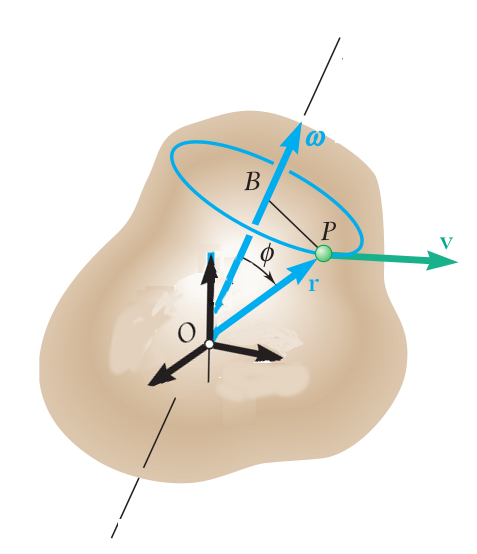
\includegraphics[width=15em]{phy_005_basics_14.png}

Üstteki resimde [8, sf. 920] eksen $\bar{w}$ vektörü etrafında olarak
gösterildi, ve açısal hızın büyüklüğü ise $\bar{w}$ vektörünün büyüklüğüne eşit,
yani $|\bar{w}|$.  Açısal hız en basit halde alttaki şekilde hareketle
anlaşılabilir, $\theta$ açısının katettiği çembersel mesafe $r\theta$'dir, eğer
zamansal $\theta(t)$ biliniyorsa, $\omega = \dot{\theta}$ bize açısal hızı, ve
$v = r\omega$ ise teğetsel hız $v$'yi verir.

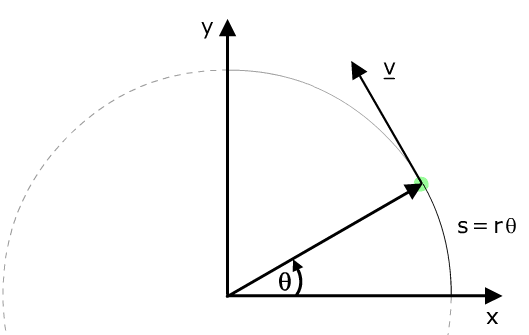
\includegraphics[width=15em]{phy_005_basics_15.png}

Üç boyutlu ortamda $v$ ve $r$ iki üstteki resimde görüldüğü üzere birer vektör
olur, bu durumda açısal hız $v$'yi, daha doğrusu $\bar{v}$ vektörünü
hesaplamanın bir diğer yolu,

$$
\bar{v} = \bar{\omega} \times \bar{r}
$$

çapraz çarpımıdır. Bu nasıl oldu? Yine iki üstteki resme bakarsak hız için önce
bize yarıçap lazım, semboller karışmasın artık yarıçap $r$ değil, $\bar{r}$
vektörü direk parçacığın yerine işaret ediyor, yarıçap $BP$ çizgisi. O çizgini
uzunluğu [6, sf. 10] ($r$ değerini $\bar{r}$'nin uzunluğu olarak alalım) şu
formül değil mi? $r\sin\phi$. Evet. O zaman $\omega$ açısal hızı ile çarparsak,
açısal hız vektörü büyüklüğünü

$$
|\bar{v}| = r \sin\phi \omega
$$

Bu bize bir büyüklük tabii, hala vektörsel değil. Peki bu büyüklüğü bir vektöre
nasıl çeviririz?  Açısal hızın yönünü birim vektör olarak kullansak?  Evet, bu
yönün her zaman $\bar{r}$ ve $\bar{\omega}$ vektörlerinin oluşturduğu düzleme
dik olacağını biliyoruz, bu bize çapraz çarpım işlemini hatırlatmalı, o zaman

$$
\bar{v} = r \sin\phi \omega
\left( \frac{\bar{\omega} \times \bar{r}}{| \bar{\omega} \times \bar{r} |}  \right)
$$

Daha basitleştirme yapmak mümkün, [7]'den hatırlarsak,
$|\bar{\omega} \times \bar{r} | = \omega r \sin\phi$, üstte yerine koyarsak,

$$
 = r \sin\phi \omega
\left( \frac{\bar{\omega} \times \bar{r}}{\omega r \sin\phi}  \right)
$$

$$
 = \bar{\omega} \times r
$$

Peki $\bar{\omega} \times r$ formülünden $\vec{v}$'yi geri elde etmek mümkün mü?

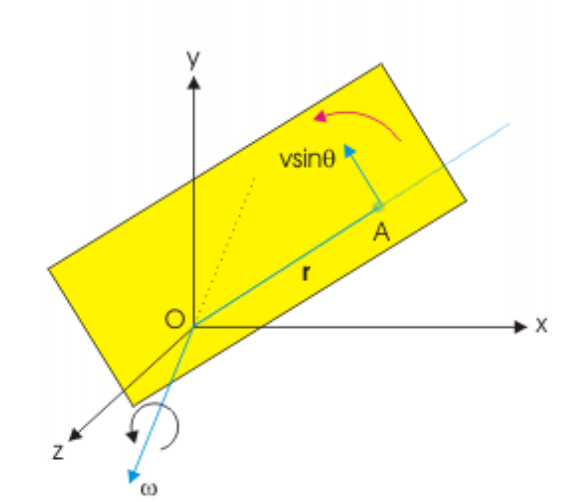
\includegraphics[width=15em]{phy_005_basics_16.png}

Üstteki resme uygun durumlar için, $\bar{\omega}$ parçacık $\vec{r}$'sinin
oluşturduğu çemberin düzleminden yukarı çıkıyor,


$$ \bar{v} = \bar{\omega} \times r
$$

İki tarafı soldan $\bar{r}$ ile çapraz çarpalım,

$$
\bar{r} \times \bar{v} = \bar{r} \times (\bar{\omega} \times r)
$$

Sağ taraf üzerinde ``BAC-CAB açılımı'' denen tekniği uygulayabiliriz,
hatırlarsak, lineer cebirde

$$
A \times (B \times C) = B(A \cdot C) - C(A \times B)
$$

Buna göre [9]

$$
= \bar{\omega} (\bar{r} \cdot \bar{r}) - \bar{r}(\bar{r} \cdot \bar{\omega})
$$

$\bar{r}$ ve $\bar{\omega}$ birbirine dik olduğuna göre noktasal çarpımları
sıfırdır. $|\bar{r}|^2 = \bar{r} \cdot \bar{r}$, o zaman

$$
\bar{r} \times \bar{v}  = \bar{\omega} |\vec{r}|^2
$$

$$
\bar{\omega}  = \frac{\bar{r} \times \bar{v}}{|\vec{r}|^2} 
$$

Açısal Momentum

Bir parçacığın açısal momentumu onun lineer momentumuna benzer şekilde
hesaplanır, lineer durumda $m \vec{v}$ hesabını yapıyoruz. Açısal durumda kütle
$m$ yerine dönme direnci $I$ kullanılacaktır, hız ise açısal hız $\vec{\omega}$
olacaktır. Acisal momentum $\vec{L}$,

$$
\vec{L} = I \vec{\omega}
$$

$\vec{L}$ ve $\vec{\omega}$'nin aynı yöne işaret ettiğine dikkat. Bir parçacık 
için $I = r^2 m$ olur, $\vec{\omega} = (\vec{r} \times \vec{v}) / r^2$ biraz
önce gördüğümüz gibi. O zaman

$$
L = (r^2 m) \left( \frac{\vec{r} \times \vec{v}}{r^2}  \right)
$$

$$
= m (\vec{r} \times \vec{v})
$$

$$
L = \vec{r} \times m\vec{v}
$$

$m\vec{v}$ ifadesi cogunlukla $\vec{p}$ ile gosterilir [5], o zaman

$$
\vec{r} \times \vec{p}
$$

Aynen momentumun zamansal türevinin bir lineer kuvvet sonucunu vermesi gibi
açısal momentumun zamansal türevi tork olacaktır [10, sf. 90]. Vektör işaretini
yazmadan,

$$
\dot{L} = \frac{\ud }{\ud t} (r \times p)  =
(\dot{r} \times p) + (r \times \dot{p})
$$

Bir numara yapalım, hızı $v = \frac{\ud r}{\ud t} = \dot{r}$ olarak ta
gösterebiliriz, çünkü $r$'nin zamansal değişimi hızdır, bu durumda üstte
eşitliğin sağ tarafındaki $p$ yerine $m\dot{r}$ koyabiliriz, ve bakıyoruz ki
$\dot{r}$ ile $m\dot{r}$ gibi iki paralel vektörün çapraz çarpımını alıyoruz, bu
tür bir çarpım sıfıra eşittir, iptal olur. Ayrıca $\dot{p}$ yerine parçacık
üstüne etki eden tüm kuvvetleri alırsak, $F$ diyelim, yeni denklem,

$$
\dot{L} = r \times F
$$

olacaktır. 


Kaynaklar

[1] Resnick, Fundamentals of Physics, 8th Ed

[2] Heuvel, {\em Pool Hall Lessons: Fast, Accurate Collision Detection Between Circles or Spheres},
    \url{https://www.gamasutra.com/view/feature/131424/pool_hall_lessons_fast_accurate_.php?print=1}

[3] Wikipedia, {\em Elastic collision}, \url{https://en.wikipedia.org/wiki/Elastic_collision}

[4] Masson, {\em Elastic Collisions in 3D}, \url{https://exploratoria.github.io/exhibits/mechanics/elastic-collisions-in-3d/index.html}

[5] Wikipedia, {\em Angular Momentum}
    \url{https://en.wikipedia.org/wiki/Angular_momentum}

[6] Schaub, {\em Analytical Mechanics of Space Systems}

[7] Bayramli, {\em Cok Degiskenli Calculus, Ders 2}

[8] Beer, {Vector Mechanics for Engnineers}

[9] Stackexchange, \url{https://physics.stackexchange.com/questions/292822/how-to-derive-the-formula-for-angular-velocity-in-three-dimensions}

[10] Taylor, {\em Classical Mechanics}

\end{document}



